\documentclass{article}
\usepackage{graphicx} % Required for inserting images
\usepackage{varwidth}
\usepackage{xcolor}
\usepackage{listings}

\definecolor{codegreen}{rgb}{0,0.6,0}
\definecolor{codegray}{rgb}{0.5,0.5,0.5}
\definecolor{codepurple}{rgb}{0.58,0,0.82}
\definecolor{backcolour}{rgb}{0.95,0.95,0.92}

\lstdefinestyle{CStyle}{
	language=C++,
	backgroundcolor=\color{backcolour},   
	commentstyle=\color{codegreen},
	keywordstyle=\color{magenta},
	numberstyle=\tiny\color{codegray},
	stringstyle=\color{codepurple},
	basicstyle=\ttfamily\footnotesize,
	breakatwhitespace=false,         
	breaklines=true,                 
	keepspaces=true,                 
	numbers=left,       
	numbersep=5pt,                  
	showspaces=false,                
	showstringspaces=false,
	showtabs=false,                  
	tabsize=2,
}
\lstset{style=CStyle}

\title{Lab 1 Report \\ \large EEL4742C - 00446}
\author{Yousef Awad}
\date{September 2025}
\setcounter{secnumdepth}{0}

\begin{document}

\maketitle
\tableofcontents
\newpage

\section{1.0 Introduction}
This lab has us exploring a totally new (very new, never been done before ever) method of pushing to the MSP430 via Code Composer Studio as well as to try and control the LEDs it has (this also never has been done until this lab, I swear).
\newline
This experiment helped us build the confidence and comprehension of the topics covered in the lecture while also letting us build familiarity with the design chocies/logic behind developing embedded systems.

\section{1.1 Documentation}
The first resources that were provided to us within the experiment was the MSP430-FR6989 development board documentation via the Lab Manual. 
\newline
Alongside the board documentation we were also given the Family User's Guide which specifically explained and showed the diagrams of the components in the MSP430. Alongside this we were also given the Chip's Data Sheet which gives out the pinout configuration of all the GPIO's and LEDs and other things connected to the MSP430 that we can use via the already written by the TI dev team.

\section{1.2 Flashing the LED}
For flashing the LEDs we first had to figure out the Code Composer Studio (CCS) works. First, we have to create a new project via File $\rightarrow$ New Project. After this we then use a blank project so that CCS doesn't do any thingy-majigs that break the code (As I had to debug this entire thing when I accidentally did that on my laptop...). To code this thing up we first have to disable the watchdog timer so that the system doesn't hang (aka it will think the program is constantly crashing and keep on reestarting it). After this we declare a variable for the loop counters, as well as set up the GPIO pins via the P1DIR and P1OUT, with P1DIR being set to output for the red LED as well as to turn it off by default. After this we then do an infinite loop followed by the internal loop that cycles through 200,000 additions (or approximaately 0.312 seconds) before toggling the red LED on and off.
\newline
Now go to the next page for the graphic of the registers...
\newpage
\hspace*{-145pt}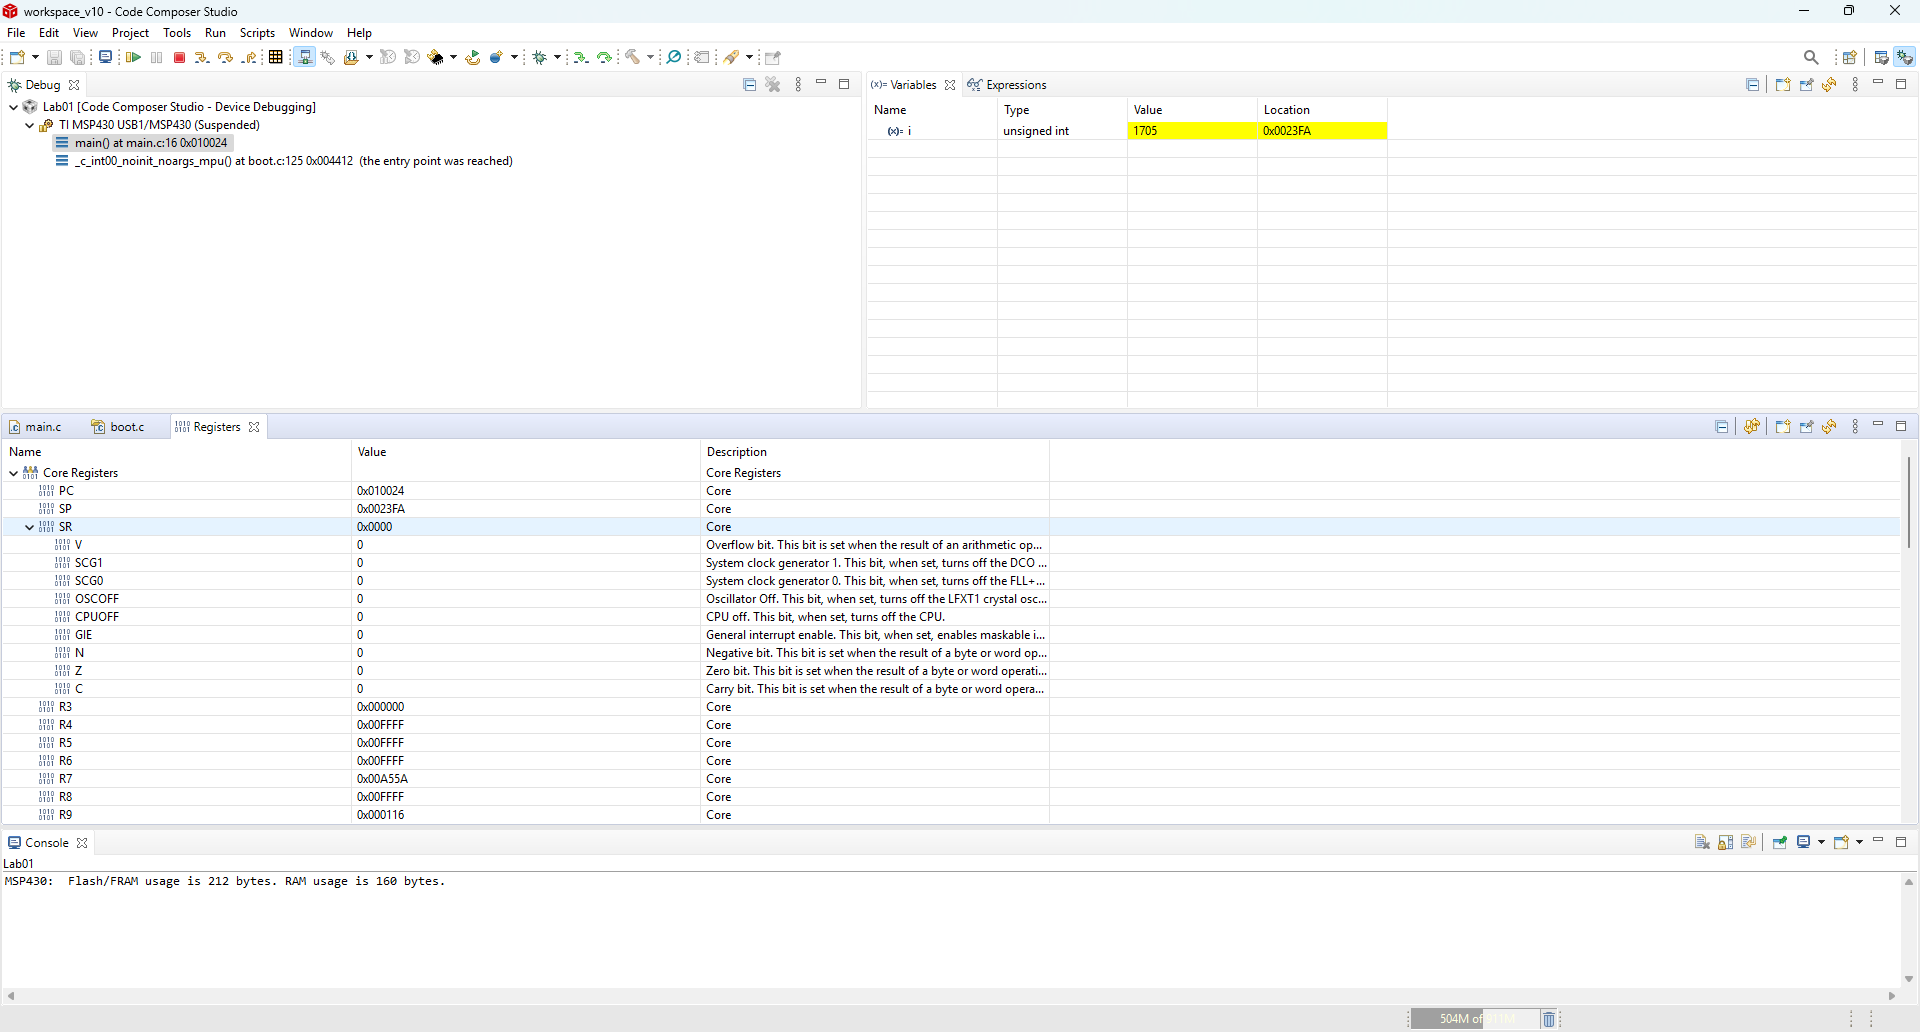
\includegraphics[width=1.75\textwidth]{pictures/1_1.png}
\newline
As well as here's the code!!
\begin{lstlisting}
// Code that flashes the red LED
#include <msp430fr6989.h>
#include <stdint.h> // for uint32_t

#define redLED BIT0 // P1.0
#define greenLED BIT7 // P9.7

void main(void)
{
    volatile uint i;
    WDTCTL = WDTPW | WDTHOLD; // Stop the Watchdog timer
    PM5CTL0 &= ~LOCKLPM5; // Disables GPIO power on by default to high impedance

    P1DIR |= redLED;
    P1OUT &= ~redLED;

    for(;;)
    {
        for(i=0; i<20000; i++) // Generates a delay of ~0.312 seconds
        {
						P1OUT ^= redLED; // Toggle the led via xor
        }
    }
}
\end{lstlisting}

\section{1.3 Flashing Two LEDs}
Now we were told by the lab manual to code up 2 flashing leds!!!!!!! WOWWWWWW. To do this I simply updated the code above to add in the Green LED in P9 as well as found the schematic for the LED Controller proper!
\begin{lstlisting}
// Code that flashes the red LED
#include <msp430fr6989.h>
#include <stdint.h> // for uint32_t

#define redLED BIT0 // P1.0
#define greenLED BIT7 // P9.7

void main(void)
{
    volatile uint i;
    WDTCTL = WDTPW | WDTHOLD; // Stop the Watchdog timer
    PM5CTL0 &= ~LOCKLPM5; // Disables GPIO power on by default to high impedance

    P1DIR |= redLED;
    P1OUT &= ~redLED;

    for(;;)
    {
        for(i=0; i<20000; i++) // Generates a delay of ~0.312 seconds
        {
						P1OUT ^= redLED; // Toggle the led via xor
        }
    }
}
\end{lstlisting}
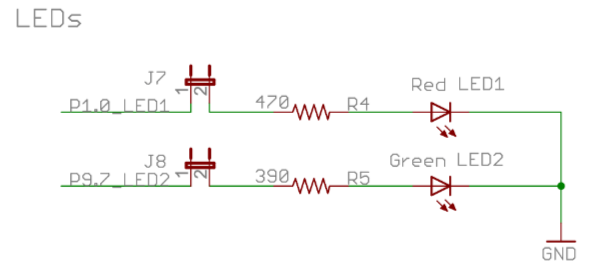
\includegraphics[width=\textwidth]{pictures/1_2.png}

\section{1.4 Setting a Long Delay}
Now we were told to make the delay longer! BUT, we have glaring problem. That problem????? It's the fact that we accidentally used a 16 bit unsigned integer for our loop counter... BUT the lab manual wants me to make a VERY VERY long delay. To fix this, we can simply either... use a 32 bit unsigned integer ORRRR simply use the \_delay\_cycles function that just tells the CPU "YOOOOO, YOU GOTTA STOP NOW", and it stops for that long... Below, I shall show both answers...
\newline
\begin{lstlisting}
// Code that flashes the red LED
#include <msp430fr6989.h>
#include <stdint.h> // for uint32_t

#define redLED BIT0 // P1.0
#define greenLED BIT7 // P9.7

void main(void)
{
    volatile uint32_t i; // solution 2
    WDTCTL = WDTPW | WDTHOLD; // Stop the Watchdog timer
    PM5CTL0 &= ~LOCKLPM5; // Disables GPIO power on by default to high impedance

    P1DIR |= redLED;
    P1OUT &= ~redLED;

    P9DIR |= greenLED; // Direct pin as output
    P9OUT &= ~greenLED; // Turns led off

    for(;;)
    {
        P9OUT ^= greenLED; // This makes it out of sync
        // Solution 2
        // for(i=0; i<200000; i++) // Generates a delay of ~3.12 seconds
        // {
        //     // Nothing, for delay
        // }
        // solution 3
        _delay_cycles(3000000); // 3*10^6 cycle stop or 3 seconds worth
        P1OUT ^= redLED; // Toggle the led via xor
        P9OUT ^= greenLED; // In-sync
    }
}
\end{lstlisting}

\section{1.5 Designing the Firetruck LED Patterns}
For this one, we were told to make two fire truck patterns (because we like fire trucks and not ambulances. OK!!!!!!) and are only told to just give you the code.
\newline
\begin{lstlisting}
// Code that is Fire Truck Pattern 1
#include <msp430fr6989.h>
#include <stdint.h> // for uint32_t

#define redLED BIT0 // P1.0
#define greenLED BIT7 // P9.7

void main(void)
{
    volatile uint32_t i; // solution 2
    WDTCTL = WDTPW | WDTHOLD; // Stop the Watchdog timer
    PM5CTL0 &= ~LOCKLPM5; // Disables GPIO power on by default to high impedance

    P1DIR |= redLED;
    P1OUT &= ~redLED;

    P9DIR |= greenLED; // Direct pin as output
    P9OUT &= ~greenLED; // Turns led off

    for (;;)
    {
        int j;
        int k;
        for (k = 0; k < 2; k++)
        {
            for (j = 0; j < 8; j++)
            {
                P1OUT ^= redLED;
                _delay_cycles(31250);
            }
            for (j = 0; j < 8; j++)
            {
                P9OUT ^= greenLED;
                _delay_cycles(31250);
            }
        }
        for (k = 0; k < 2; k++)
        {
            // half
            for (j = 0; j < 8; j++)
            {
                P1OUT ^= redLED;
                _delay_cycles(62500);
            }
            for (j = 0; j < 8; j++)
            {
                P9OUT ^= greenLED;
                _delay_cycles(62500);
            }
        }
    }
}
\end{lstlisting}
\newpage
\begin{lstlisting}
// Code that shows Fire Truck Pattern 2
#include <msp430fr6989.h>
#include <stdint.h> // for uint32_t

#define redLED BIT0 // P1.0
#define greenLED BIT7 // P9.7

void main(void)
{
    volatile uint32_t i; // solution 2
    WDTCTL = WDTPW | WDTHOLD; // Stop the Watchdog timer
    PM5CTL0 &= ~LOCKLPM5; // Disables GPIO power on by default to high impedance

    P1DIR |= redLED;
    P1OUT &= ~redLED;

    P9DIR |= greenLED; // Direct pin as output
    P9OUT &= ~greenLED; // Turns led off

    for (;;)
    {
        int j;
        for (j = 0; j < 8; j++)
        {
            P9OUT ^= greenLED; // This makes it out of sync
            _delay_cycles(500000); // 3*10^6 cycle stop or 3 seconds worth
            P1OUT ^= redLED; // Toggle the led via xor
        }
        for (j = 0; j < 8; j++)
        {
            P9OUT ^= greenLED; // This makes it out of sync
            _delay_cycles(250000); // 3*10^6 cycle stop or 3 seconds worth
            P1OUT ^= redLED; // Toggle the led via xor
        }
        for (j = 0; j < 8; j++)
        {
            P9OUT ^= greenLED; // This makes it out of sync
            _delay_cycles(125000); // 3*10^6 cycle stop or 3 seconds worth
            P1OUT ^= redLED; // Toggle the led via xor
        }

        P9OUT &= ~greenLED; // Turns green off
        P1OUT &= ~redLED; // Turns red off

        // On then off 3 times
        for (j = 0; j < 8; j++)
        {
            P9OUT ^= greenLED;
            P1OUT ^= redLED;
            _delay_cycles(250000);
        }
    }
}
\end{lstlisting}

\section{Student Q\&A}
\subsection{Q1}
\textbf{Given: } In this lab, we used a delay loop to create a small delay; what is its effect on the battery life if the device is battery operated? Is it a good way of setting delays?
\\
\\
Using a delay/for loop for the small delay is honestly a terrible idea, due to the fact that it is having to compute the additions of the amount of times that it loops and therefore wastes energy doing addition cycles that are unneeded when you can simply use the \_delay\_cycles function instead.

\subsection{Q2}
\textbf{Given: } The MSP430 CPU clock can be configured to multiple frequencies via software. What happens to the delay generated by the delay loop if the CPU clock frequency is changed?
\\
\\
If the frequency of the clock changes, the delay loop will also change due to the fact that the delay is reliant on the amount of cycles, OR, the amount of additions PER cycle that it computes.

\subsection{Q3}
\textbf{Given: } How does the code run in the debug mode? Is the microcontroller running as an independent computer?
\\
\\
In debug mode, the code runs in tandem to the computer you are on, and therefore cannot be run as an independent computer.

\subsection{Q4}
\textbf{Given: } How does the code run in the normal mode? Is the microcontroller running as an independent computer?
\\
\\
In normal mode, the code runs seperate to the computer you used to push the code, and therefore means it is running as an independent computer.

\subsection{Q5}
\textbf{Given: } In which mode does the reset button work?
\\
\\
The Reset button only works when you are in normal mode. It \textit{does not} work in debug mode.

\subsection{Q6}
\textbf{Given: } What is the data type uint16 t ? What about int16 t ? Are these standard C syntax?
\\
\\
The data type of uint16\_t is an unsigned integer of bit length 16. int16\_t is the signed integer variant again with 16 bit length. These are not in the standard C \textit{syntax}, BUT can be included as a module as it is part of the C standard \textit{library} just like stdio or stdstring.

\section{Conclusion}
To sum it all up, this lab was a perfect introduction to using the MSP430-FR6989 as well as the Code Composer Studio software stack. It provided me with experience on how to push code to the board, as well as finely control the LEDs using logical operators to set individual bits on and off on a given register. My only complaint for this lab is that the videos for the Fire Truck portion were hard to watch and it was also frustrating to try and guesstimate what they were doing without being able to slow down the video. I do recommend for next time uploading them as a video proper so that future student have the ability to slow down the video and accurately be able to see the changes to the LEDs.

\end{document}
